\documentclass[varwidth=true,crop=false]{standalone}
\usepackage[chatter]{rotating}
\usepackage{amssymb,amsmath}
\usepackage{pgfplots}

\usepackage{geometry}
\geometry{
paperwidth=8in,
paperheight=6.25in,
margin=0.25in
}

\newcommand{\pisub}[1]{\pi_{\mathrm{#1}}}
\newcommand{\pilow}{\pisub{low}}
\newcommand{\pihigh}{\pisub{high}}
\newcommand{\piI}{\langle \pisub{I} \rangle}
\newcommand{\piS}{\langle \pisub{S} \rangle}
\newcommand{\ledger}{\bar\pi_{ib}}

\newcommand{\meanvar}[1]{\langle #1 \rangle}
\newcommand{\meansl}{\meanvar{s}}
\newcommand{\meanpi}{\meanvar{\pi}}
\newcommand{\meansoc}{\meanvar{\pi_\mathrm{S}}}
\newcommand{\meanasoc}{\meanvar{\pi_\mathrm{A}}}
\newcommand{\meanT}{\meanvar{T}}

\newcommand{\bandit}{\text{Bandit}_b(0, 1)}

\begin{document}

    \begin{minipage}{3.75in}
      \centering
      {\hspace{5.25em}\huge $B = 2$}
    \end{minipage}%
    \begin{minipage}{3.75in}
      \centering
      {\hspace{2.0em}\huge $B = 10$}
    \end{minipage}~\\

    \begin{minipage}{3.75in}
    \begin{rotate}{90}
      {\parbox{2.5in}{
          \centering
          \vspace{-2.5em} {\huge$ \pilow = 0.1$} \\
          {\begin{rotate}{-90}{\huge $\frac{\meanT}{L}$}\hspace{3em}\end{rotate}}
      }}
    \end{rotate}%
    \hspace{2em}
      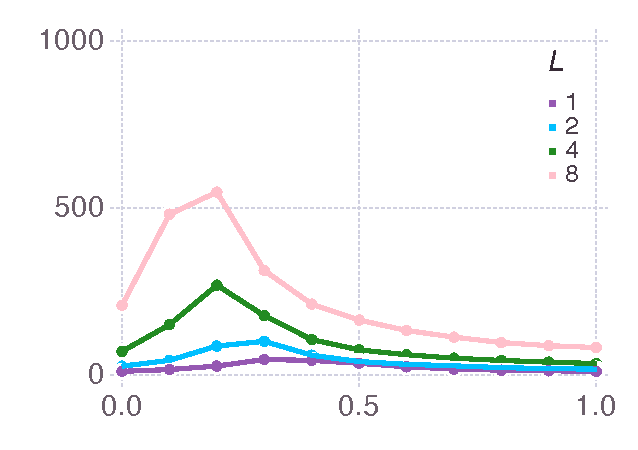
\includegraphics[width=\textwidth]{Figures/step_over_u_lowpayoff=0.1_nbehaviors=2.pdf}
    \end{minipage}\noindent\begin{minipage}{3.75in}%
      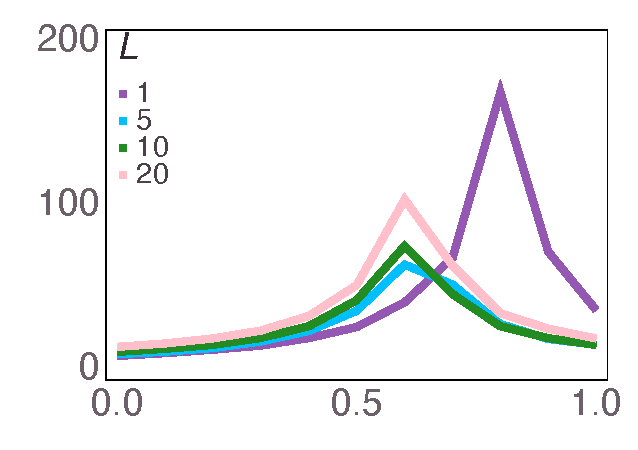
\includegraphics[width=\textwidth]{Figures/step_over_u_lowpayoff=0.1_nbehaviors=10.pdf}
    \end{minipage}~\\[0.5em]

    \begin{minipage}{3.75in}
    \begin{rotate}{90}
      {\parbox{2.5in}{
          \centering
          \vspace{-2.5em} {\huge$ \pilow = 0.45$} \\
          {\begin{rotate}{-90}{\huge $\frac{\meanT}{L}$}\hspace{3em}\end{rotate}}
      }}
    \end{rotate}%
    \hspace{2em}
      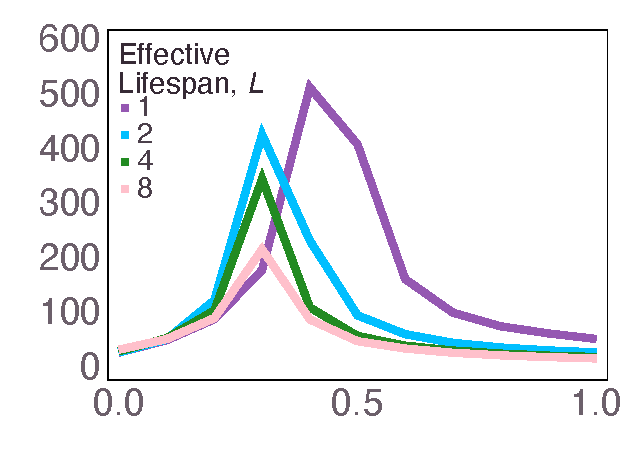
\includegraphics[width=\textwidth]{Figures/step_over_u_lowpayoff=0.45_nbehaviors=2.pdf}
        \\[-2.75em]
        \begin{center}
          {\hspace{3.25em} \huge $\quad u$}
      \end{center}
        \end{minipage}\noindent\begin{minipage}{3.75in}%
      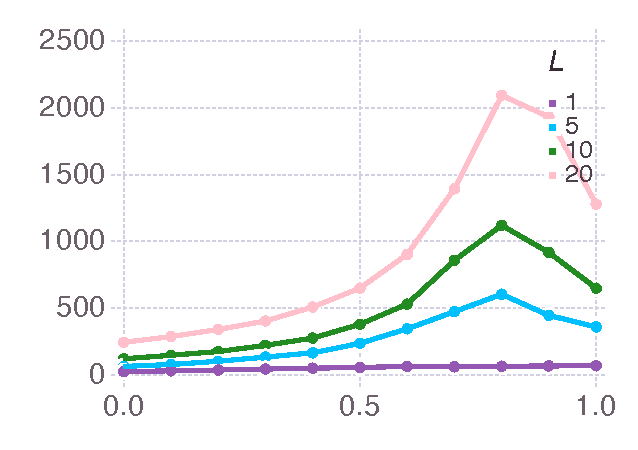
\includegraphics[width=\textwidth]{Figures/step_over_u_lowpayoff=0.45_nbehaviors=10.pdf}
      \\[-2.75em]
      \begin{center}
        {\huge $\quad u$}
      \end{center}
    \end{minipage}
\end{document}
